\section{Basic Concepts}
\subsection{Quantum bits (qubits)}

Classical bits: $0, 1$ \newline
Quantum bit \textit{qubit}: Superposition of $0$ and $1$:

A quantum state $\ket{\psi}$ is described as 
\begin{equation}
    \ket{\psi} := \alpha \ket{0} + \beta \ket{1}, \quad \alpha, \beta \in \mathbb{C} 
\end{equation}
where 
\begin{equation}
    \abs{\alpha}^2 + \abs{\beta}^2 = 1 \quad \text(normalization).
\end{equation}
%
Mathematical description: $\ket{\psi} \in \mathbb{C}^2$ with
\begin{equation*}
    \ket{0} = \begin{pmatrix}1 \\ 0 \end{pmatrix}, 
    \quad \ket{1} = \begin{pmatrix}0 \\ 1\end{pmatrix}
    \quad \leadsto \ket{\psi} = \begin{pmatrix}
        \alpha \\ \beta
    \end{pmatrix}
\end{equation*}


Different from classical bits, cannot (in general) directly observe / measure a qubit 
(the amplitudes $\alpha$ and $\beta$).
%
Instead: "\textit{standard}" measurement will result in 
\begin{itemize}
    \item $0$ with probability $\abs{\alpha}^2$
    \item $1$ with probability $\abs{\beta}^2$
\end{itemize}
%

The measurement also \underline{changes} the qubit (\textit{wavefunction collapse}).
%
If measuring $0$, the qubit will be $\ket{\psi} = \ket{0}$ directly after the measurement,
and likewise if measuring $1$, the qubit will be $\ket{\psi} = \ket{1}$. \newline

In practise: Can estimate the probabilities $\abs{\alpha}^2$ and $\abs{\beta}^2$ in 
experiments by repeating the same experiment many times (i.e via outcome statistics).
These repetitions are called \textit{trials} or \textit{shots}.

\begin{figure}[h]
    \centering
    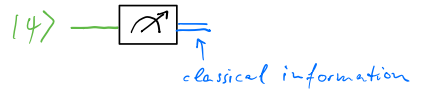
\includegraphics[scale=0.5]{chapters/res/circuit-notation.png}
    \caption{Circuit notation}
\end{figure}
\newpage

A useful graphical deputation of a qubit is the \underline{Bloch sphere} representation:
If $\alpha$ and $\beta$ happen to be real-valued, then can find angle 
$\vartheta \in \mathbb{R}$ such that
\begin{equation}
    \alpha = \cos{\frac{\vartheta}{2}}, \quad \beta = \sin{\frac{\vartheta}{2}}
\end{equation}
\begin{equation*}
    (\leadsto \abs{\alpha}^2 + \abs{\beta}^2 
    = \cos{\frac{\vartheta}{2}} + \sin{\frac{\vartheta}{2}}) = 1 \quad \color{green}\checkmark
\end{equation*}

\begin{figure}[h]
    \centering
    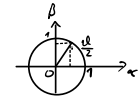
\includegraphics[scale=0.5]{chapters/res/bloch_sphere_sin_cos.png}
\end{figure}

In general: represent 
\begin{align*}
    \alpha &= e^{i \gamma} \cos{\frac{\vartheta}{2}} \\
    \beta &= e^{i (\varphi + \gamma)} \sin{\frac{\vartheta}{2}} \\
\end{align*}
using so-called phase angles $\gamma$ for $\alpha$ and $\varphi + \gamma$ for $\beta$.

\begin{figure}[h]
    \centering
    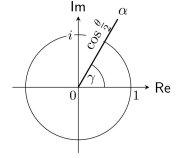
\includegraphics[scale=0.6]{chapters/res/sin-cos-complex.png}
\end{figure}

Then:
\begin{align}
    \ket{\psi} &= 
        e^{i \psi} \cos{\frac{\vartheta}{2}} \cdot \ket{0} 
        + \underbrace{e^{i (\varphi + \gamma)}}_{= \text{ } e^{i\varphi} \cdot e^{i\gamma}} \sin{\frac{\vartheta}{2}} \cdot \ket{1} \\
        %
        &= \underbrace{e^{i \gamma}}_{\text{can be ignored here}}
        \left(\cos{\frac{\vartheta}{2}} \cdot \ket{0} + e^{i\varphi} \cdot \sin{\frac{\vartheta}{2}} \cdot \ket{1}\right)
\end{align}

Thus $\ket{\psi}$ is characterized by two angles $\varphi$ and $\gamma$;
these specify the point defined as 
\begin{equation*}
    \vec{r} = \begin{pmatrix}
        \cos{\varphi} \cdot \sin{\vartheta} \\
        \sin{\varphi} \cdot \cos{\vartheta} \\
        \cos{\vartheta}
    \end{pmatrix}
\end{equation*}

on the surface of a sphere:
\begin{figure}[h!]
    \centering
    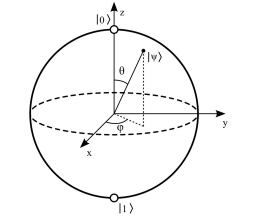
\includegraphics[scale=0.5]{chapters/res/bloch-sphere.png}
    \caption{Bloch Sphere (Felix Bloch)}
\end{figure}

\subsection{Single qubit gates}